\chapter{Линейные порядки частично упорядоченных множеств с учётом
зависимостей операций с памятью: построение и анализ}\label{sec:ch3}

В предыдущей главе было показано, что задача анализа консистентности
памяти сводится к построению всех линейных порядков частично
упорядоченного множества операций с памятью. Однако прямое решение
этой задачи сталкивается с комбинаторным взрывом: количество порядков
растёт экспоненциально, а в худшем случае — факториально
(см.~разделы~\ref{sec:ch2/linext-count}–\ref{sec:ch2/topoalg-comp}). Это
делает полный перебор непригодным для программ с большим числом
обращений к памяти.

Ключевая идея главы состоит в том, что не все линейные порядки
приводят систему в различные состояния. Многие перестановки
эквивалентны с точки зрения результата исполнения, что позволяет
сократить пространство поиска.

В разделе~\ref{sec:ch2/indep} рассматривается учёт независимости:
вводятся классы эквивалентных перестановок и алгоритмы топологической
сортировки, исключающие эквивалентные порядки. В
разделе~\ref{sec:ch2/dep} предлагается учёт зависимостей: алгоритм
обхода, направляющий неориентированные рёбра зависимости и
порождающий бинарное дерево порядков. В
разделе~\ref{sec:ch2/indep-dep} проводится сравнение алгоритмов
и показывается, что учёт классов эквивалентности существенно
сокращает количество анализируемых порядков.

\section{Учёт независимости операций при анализе линейных порядков в
многопоточных программах}
\label{sec:ch2/indep}

Основной проблемой как при анализе многопоточных программ, так и при
построении всевозможных линейных перестановок, является отсутствие
оптимального решения.

Задача поиска линейных порядков относится к классу $\#P$-полных задач
(см.~\cite{linextcount}). Количество линейных порядков и сложность
алгоритма их обхода может достигать $n!$, как видно из
формул~\eqref{eq:topo-comp-lims-p0}
и~\eqref{eq:linext-count-lims-p0}. Полное построение и анализ такого
объёма частичных порядков становится затруднительным для больших значений $n$.

Однако операции с памятью, являющиеся предметом настоящего
исследования, обладают дополнительными свойствами, которые могут быть
учтены при построении линейных порядков. Одним из таких свойств
является независимость операций.

Назовём две операции с памятью $A$ и $B$ \textbf{независимыми}, если
исполнение операций в порядке $A$--$B$ приводит систему в такое же
состояние, как и исполнение операций в порядке $B$--$A$. Аналогично,
\textbf{последовательность} $\{A\text{--}B\}$ называется
\textbf{независимой} относительно операции $C$, если исполнение
$A$--$B$--$C$ приводит к тому же состоянию, что и исполнение $C$--$A$--$B$.

Операции (a), (b), (c) и (d) из листинга~\ref{lst:indep} являются
независимыми, так как любой порядок их исполнения приводит к одним и
тем же значениям переменных X, Y, Z и K. В данном конкретном
примере не имеет значения, были ли эти операции выполнены в одном
потоке или в нескольких потоках.

\begin{minipage}{\textwidth}
  \centering
  \lstinputlisting[caption={Пример независимых операций}, label={lst:indep},
  captionpos=b]{src/indep.txt}
\end{minipage}

Различные порядки исполнения независимых операций приводят систему в
неразличимые состояния. Это означает, что при анализе корректности
исполнения программы такие порядки не требуется рассматривать по
отдельности: достаточно проанализировать лишь один представитель от
каждого множества порядков, дающих одинаковый результат.
В предельном случае, когда все операции в программе независимы,
вместо $n!$ различных линейных порядков достаточно рассмотреть лишь один.

\subsection{Классы эквивалентных перестановок}
\label{sec:ch1/eqiv-cl}

Рассмотрим множество всевозможных линейных перестановок $S_n$. Две
перестановки из $S_n$ называются эквивалентными, если одна может быть
получена из другой путём замены некоторой подпоследовательности
элементов на ту же подпоследовательность, но с элементами,
переставленными определённым образом. Обобщённая теория таких
преобразований представлена в работах~\cite{knuth,dual,representation}.

Например, перестановка $12\textbf{345}6$ может быть преобразована в
$12\textbf{543}6$ путём замены подпоследовательности \textbf{345} на
подпоследовательность \textbf{543}. Можно сказать, что $123456$
эквивалентна $125436$ относительно замены $123 \leftrightarrow 321$.
Или, используя нотацию множеств: перестановки эквивалентны
относительно $\{123, 321\}$.

Пусть $\pi \in S_n$ и пусть $B = \{B_1, \dots, B_t\}$ — заданное
разбиение $S_k$, где $k \le n$. Каждый элемент $B_l$ является
шаблоном длиной $k$, относительно которого допускается перестановка
элементов. Назовём две перестановки \textbf{$B$-эквивалентными}, если
одна может быть получена из другой путём последовательного применения
перестановок, при которых каждая перестановка $\sigma_i$ шаблона
производится с теми же элементами $\sigma_j$ шаблона, а $\sigma_i$ и
$\sigma_j$ принадлежат одному и тому же множеству $B_l$. Тогда
$Eq(\pi, B)$ обозначает множество перестановок, эквивалентных $\pi$
относительно $B$.

Таким образом, $125436 \in Eq(123456, \{\{123, 321\}\})$.

Ограничим дальнейшее исследование перестановками только соседних
элементов. Обозначим через $B^{|}$ отношение эквивалентности, а через
$Eq^{|}(\pi, B)$ — класс эквивалентности перестановки $\pi$ с учётом
замены $B$ только для соседних элементов. То есть $2134 \in
Eq^{|}(1234, \{\{123, 213\}\})$.

\subsection{Построение классов независимости многопоточной программы}
\label{sec:ch2/construction-indep}

Построение всех возможных GMO может оказаться избыточным, особенно
когда в рассматриваемой программе присутствуют независимые операции.
Если два различных GMO отличаются только перестановкой независимых
операций, то такие порядки приводят систему в одно и то же
неразличимое состояние. В этом случае достаточно построить и
проанализировать лишь один представитель такого порядка.

В уравнении~\eqref{eq:B-indep} задано построение разбиений,
относительно которых допускается перестановка элементов:
\begin{equation}
  \forall \{x, y\} \in Prog \mid x, y \text{ — независимые}
  \rightarrow \{xy, yx\} \in B^|.
  \label{eq:B-indep}
\end{equation}

Пусть $\tau \in Eq(\pi, B^|)$. Тогда $\tau = \dots xy \dots$, а $\pi
= \dots yx \dots$. Поскольку $x$ и $y$ являются независимыми
операциями, и любой порядок их исполнения приводит систему в одно и
то же состояние, достаточно рассмотреть только один порядок,
принадлежащий данному классу эквивалентности. Учёт этого свойства при
построении дерева всевозможных линейных порядков позволяет
существенно уменьшить количество ветвей, требующих полного построения.

Многопоточная программа полностью задаёт отношение $B^|$ в
соответствии с формулой~\eqref{eq:B-indep}. Поскольку все линейные
порядки внутри одного класса эквивалентности приводят систему в одно
и то же наблюдаемое состояние, достаточно построить все различные
классы эквивалентности $Eq(\pi, B^|)$.

\subsection{Топологическая сортировка с учётом независимости}
\label{sec:ch2/topo-indep}

Для учёта независимости перестановок введём дополнительные параметры
в алгоритм~\ref{alg:topo}.

\begin{algorithm}[H]
  \caption{Обход частично упорядоченного множества с учётом независимости}
  \label{alg:topo-indep}
  \begin{algorithmic}[1]
    \Require $P$ -- частично упорядоченное множество.
    \Require $B^{|}$ -- разбиение из независимых элементов.
    \Require $\mathcal{B} = \{B_n\}$, где $B_n$ -- множество из
    разбиений на $n$-ом шаге рекурсии. $\mathcal{B}(n) = B_n$
    \Require $\pi$ — текущий линейный порядок.
    \Require $y$ — вершина, обработанная на предыдущем шаге рекурсии.
    \Require $ctx$ — контекст алгоритма обхода.
    \Function{Traverse}{$P$, $B^{|}$, $\mathcal{B}$, $\pi$, $y$, $ctx$}
    \If{$P = \emptyset$}
    \State $L(P) \gets \pi \cup L(P)$ \Comment{Полностью построили
    линейный порядок}
    \EndIf
    \State $n \gets |\pi|$
    \State $\mathcal{B}(n) \gets \emptyset$
    \ForAll{$\forall x \in \min(P) \mid \{xy, yx\} \not \in
    \mathcal{B}(n-2)$} \label{alg:line:l5}
    \State \Call{Process}{$ctx$, $\pi$, $x$} \Comment{Обработка
    элемента множества}
    \State \Call{Traverse}{$P \setminus \{x\}$, $B^{|}$,
    $\mathcal{B}$, $\pi \stackrel{add}{\longleftarrow} x$, $x$, $ctx$}
    \If{$\{xy, yx\} \in B^{|}$}
    \State $\mathcal{B}(n-2) \gets \{xy, yx\} \cup \mathcal{B}(n-2)$
    \label{alg:line:l9}
    \EndIf
    \EndFor
    \EndFunction
  \end{algorithmic}
\end{algorithm}

В алгоритме~\ref{alg:topo-indep} производится дополнительный учёт
обработанных независимых порядков, чтобы избежать обработки их
эквивалентных перестановок. На строке~\ref{alg:line:l5} из цикла исключаются
минимальные элементы, перестановка которых с элементом на предыдущем
шаге уже была обработана. На строке~\ref{alg:line:l9} обновляется информация об
обработанных парах независимых элементов.

Рассмотрим полученное дерево линейных порядков
(рис.~\ref{fig:topo-trav-indep-tree}) на том же примере, что и на
рисунке~\ref{fig:topo-trav}. Дополнительно обозначим вершины $\{2,
4\}$ и $\{2, 5\}$ как независимые: $B^| = \{\{24, 42\}, \{25,
52\}\}$. На рисунке~\ref{fig:topo-indep-poset} рёбра независимости
обозначены двойной чертой.

\begin{figure}[htbp]
  \centerfloat{
    \begin{tikzpicture}[
    node distance=1.5cm and 1cm,
    stepnode/.style={rectangle, draw=black, dashed, thick, inner sep=5pt, rounded corners=5pt},
    dag/.style={circle, draw=black, fill=white, inner sep=2pt, minimum size=8mm},
    arrow/.style={-stealth, thick}
]
    \node[dag] (1-1) {1};
    \node[dag, below left=0.5cm of 1-1] (1-2) {2};
    \node[dag, right=1.0cm of 1-1] (1-3) {3};
    \node[dag, below left=0.5cm of 1-3] (1-4) {4};
    \node[dag, below left=0.5cm of 1-4] (1-5) {5};

    \draw[arrow] (1-1) -- (1-2);
    \draw[arrow] (1-1) -- (1-4);
    \draw[arrow] (1-3) -- (1-4);
    \draw[arrow] (1-4) -- (1-5);

    \draw[line width=1pt, double distance=3pt] (1-2) -- (1-4);
    \draw[line width=1pt, double distance=3pt] (1-2) -- (1-5);
\end{tikzpicture}

  }
  \caption{Частично упорядоченное множество с рёбрами независимости}
  \label{fig:topo-indep-poset}
\end{figure}

\begin{figure}[htbp]
  \centerfloat{
    \tikzset{
    cross arrow/.style={
        -stealth, thick,
        postaction={
            decorate,
            decoration={
                markings,
                mark=at position 0.5 with {
                    \draw[-, red, line width=3pt]
                        (-0.15,-0.15) -- (0.15,0.15)
                        (-0.15,0.15) -- (0.15,-0.15);
                }
            }
        }
    }
}
\begin{tikzpicture}[
    node distance=1.5cm and 1.5cm,
    dag/.style={on grid, circle, draw=black, fill=white, inner sep=2pt, minimum size=8mm},
    arrow/.style={-stealth, thick}
]

\node[dag] (1-1) {1};
\node[dag, below left=1.5cm and 1.5cm of 1-1] (2-2) {2};
\node[dag, below=1.5cm of 2-2] (3-3) {3};
\node[dag, below=1.5cm of 3-3] (4-4) {4};
\node[dag, below=1.5cm of 4-4] (5-5) {5};

\node[dag, below right=1.5cm and 1.5cm of 1-1] (3-2) {3};
\node[dag, below=1.5cm of 3-2] (4-3) {4};

\node[dag, below left=1.5cm and 1.5cm of 4-3] (2-4) {2};
\node[dag, below=1.5cm of 2-4] (5-5_1) {5};

\node[dag, below=1.5cm of 4-3] (5-4) {5};
\node[dag, below=1.5cm of 5-4, draw=black!25, dashed, text=black!25] (2-5) {2};

\node[dag, right=3.0cm of 1-1] (3-1) {3};
\node[dag, below=1.5cm of 3-1] (1-2) {1};
\node[dag, below=1.5cm of 1-2] (2-3) {2};
\node[dag, below=1.5cm of 2-3, draw=black!25, dashed, text=black!25] (4-4_1) {4};
\node[dag, below=1.5cm of 4-4_1, draw=black!25, dashed, text=black!25] (5-5_2) {5};

\draw[arrow] (1-1) -- (2-2);
\draw[arrow] (2-2) -- (3-3);
\draw[arrow] (3-3) -- (4-4);
\draw[arrow] (4-4) -- (5-5);

\draw[arrow] (1-1) -- (3-2);
\draw[arrow] (3-2) -- (4-3);

\draw[arrow] (4-3) -- (2-4);
\draw[arrow] (2-4) -- (5-5_1);

\draw[arrow] (4-3) -- (5-4);
\draw[cross arrow] (5-4) -- (2-5);

\draw[arrow] (3-1) -- (1-2);
\draw[arrow] (1-2) -- (2-3);
\draw[cross arrow] (2-3) -- (4-4_1);
\draw[arrow, draw=black!25, dashed] (4-4_1) -- (5-5_2);

\draw[arrow] (3-2) -- (2-3);
\draw[arrow] (1-2) -- (4-3);

\end{tikzpicture}

  }
  \caption{Пример построенного дерева (сжатого в ОАГ) линейных
  порядков с учётом независимости}
  \label{fig:topo-trav-indep-tree}
\end{figure}

Видно, что порядки $13452$ и $31245$ не были обработаны, так как
$13452 \in Eq(13425, B^|)$ и $31245 \in Eq(31425, B^|)$.

Применение цепочки последовательных эквивалентных перестановок
порождает перестановку, эквивалентную исходной. Рассмотрим это на
примере. Пусть $B^{|} = \{\{01, 10\}, \{02, 20\}\}$ и $\pi = 012$.
Тогда $012 \stackrel{Eq(\pi, B^{|})}{=} 102 \stackrel{Eq(\pi,
B^{|})}{=} 120$. Таким образом, $012 \stackrel{Eq(\pi, B)}{=} 120$,
где $B = \{012, 120\} \cup B^{|}$.

Обобщим данное свойство.

\begin{lemma}
  Последовательными действиями переупорядочивания эквивалентных пар
  можно переставить элемент с подпорядком любой длины, если все
  элементы этого подпорядка независимы с данным элементом.
  \label{lm:n-reorder}
\end{lemma}

\begin{proof}
  Пусть $\tau = \pi x \mathrm{Y} \gamma$ — линейный порядок, такой
  что $\forall y \in \mathrm{Y} \rightarrow \{xy, yx\} \in B^|$.

  \begin{align}
    \tau & = \pi \pmb{xy} \mathrm{Y}^{'} \gamma
    \stackrel{Eq(\tau, B^|)}{=}
    \pi \pmb{yx} \mathrm{Y}^{'} \gamma
    \stackrel{Eq(\tau, B^|)}{=} \nonumber \\
    & \dots \text{так же последовательно переставляем } x \text{ со
    следующим элементом из } \mathrm{Y}^{'} \dots \nonumber \\
    & \stackrel{Eq(\tau, B^|)}{=}
    \pi y \mathrm{Y}^{'} x \gamma
    = \pi \mathrm{Y} x \gamma = \tau^{'}. \nonumber
  \end{align}
  Таким образом,
  \[
    \tau^{'} = Eq(\tau, B^| \cup \{x\mathrm{Y}, \mathrm{Y}x\}).
  \]
\end{proof}

Задача построения всевозможных разбиений из независимых элементов
также не имеет оптимального решения, и нет смысла решать её для учёта
всевозможных перестановок независимых элементов. Однако можно
дополнить алгоритм~\ref{alg:topo-indep}, чтобы учесть свойство,
представленное в лемме~\ref{lm:n-reorder}.
Алгоритм~\ref{alg:topo-indep-lookup} учитывает отброшенные ветви
исполнения, транзитивно обновляя информацию о независимых парах элементов.

\begin{algorithm}[H]
  \caption{Обход частично упорядоченного множества с учётом
  независимых последовательностей операций}
  \label{alg:topo-indep-lookup}
  \begin{algorithmic}[1]
    \Require $P$ -- частично упорядоченное множество.
    \Require $B^{|}$ -- разбиение из независимых элементов.
    \Require $\mathcal{B} = \{B_n\}$, где $B_n$ -- множество из
    разбиений на $n$-ом шаге рекурсии. $\mathcal{B}(n) = B_n$
    \Require $\pi$ — текущий линейный порядок.
    \Require $y$ — вершина, обработанная на предыдущем шаге рекурсии.
    \Require $ctx$ — контекст алгоритма обхода.
    \Function{Traverse}{$P$, $B^{|}$, $\mathcal{B}$, $\pi$, $y$, $ctx$}
    \If{$P = \emptyset$}
    \State $L(P) \gets \pi \cup L(P)$ \Comment{Полностью построили
    линейный порядок}
    \EndIf
    \State $\mathcal{B}(n) \gets \emptyset$
    \State $\mathcal{B}(n-1) \gets \mathcal{B}(n-1) \cup \{\{xz,
      zx\} \in B^{|} \mid \forall z \in P,\ \forall x \mid \{xy, yx\}
    \in \mathcal{B}(n-2)\}$
    \ForAll{$\forall x \in \min(P) : \{xy, yx\} \not \in
    \mathcal{B}(n-2)$}\label{alg:line:traverse}
    \State \Call{Process}{$ctx$, $\pi$, $x$} \Comment{Обработка
    элемента множества}
    \State \Call{Traverse}{$P \setminus \{x\}$, $B^{|}$,
    $\mathcal{B}$, $\pi \stackrel{add}{\longleftarrow} x$, $x$, $ctx$}
    \If{$\{xy, yx\} \in B^{|}$}
    \State $\mathcal{B}(n-2) \gets \{xy, yx\} \cup \mathcal{B}(n-2)$
    \EndIf
    \EndFor
    \EndFunction
  \end{algorithmic}
\end{algorithm}

Обновление множества разбиений с предыдущего шага рекурсии
$\mathcal{B}(n-1) = B_{n-1}$ позволяет не терять информацию
при отбрасывании уже обработанных элементов на
строке~\ref{alg:line:traverse}. Покажем, что данный обход реализует
свойство, сформулированное в лемме~\ref{lm:n-reorder}.

\begin{lemma}
  Алгоритм~\ref{alg:topo-indep-lookup} учитывает перестановки
  независимых последовательностей элементов.
  \label{lm:algo}
\end{lemma}

\begin{proof}
  Пусть $\tau = \pi x \mathrm{Y} \gamma$ — уже построенный линейный
  порядок, такой что $\forall y \in \mathrm{Y} \rightarrow \{xy, yx\}
  \in B^|$. Обозначим через $\mathrm{Y}^{\min}$ множество минимальных
  элементов из множества $\mathrm{Y}$. На каждом шаге рекурсии будем
  рассматривать такой $y \in \mathrm{Y}^{\min}$, чтобы сохранять
  подпорядок элементов как в $\mathrm{Y}$.

  Пусть уже построен подпорядок $\pi y$ на шаге рекурсии $n$.
  Следующими элементами в ней могут быть $x$ и $\dot{y} \in
  \dot{\mathrm{Y}}^{\min}$. Порядок $\pi y x$ не будет рассмотрен
  из-за того, что $\{xy, yx\} \in B_{n-2}$, но при этом
  $B_{n-1} = \{x\dot{y}, \dot{y}x\} \mid \dot{y} \in
  \dot{\mathrm{Y}}^{\min} = B_{(n+1) - 2}$.

  Рассмотрим следующий шаг рекурсии $n+1$, на котором уже построен
  подпорядок $\pi y \dot{y}$. Следующими элементами в ней могут быть
  $x$ и $\ddot{y} \in \ddot{\mathrm{Y}}^{\min}$. Порядок $\pi y
  \dot{y}x$ не будет рассмотрен из-за того, что $\{x\dot{y},
  \dot{y}x\} \in B_{(n+1) - 2}$. Продолжим рассуждения, пока из
  минимальных элементов не останется только $x$. Тогда порядок $\pi
  y\dot{y}\ddot{y}\dots x = \pi \mathrm{Y} x$ не будет рассмотрен.
  Что и требовалось доказать.
\end{proof}

\subsection{Асимптотика алгоритма построения всех линейных порядков
топологической сортировкой с учётом независимости}
\label{sec:ch2/topoalg-indep-comp}

Воспользуемся полученной ранее формулой~\ref{eq:topo-comp} для количества
операций:
\[
  C_N = \sum_{k=1}^{N} k \prod_{l=1}^{N-k} \frac{1-q^{k+l}}{1-q},
\]
где $q = 1 - p$, а $p$ — вероятность того, что любые два элемента $x$
и $y$ частично упорядоченного множества $P$ находятся в отношении $x <_p y$.

Введём обозначение $p_i(x, y) = p_i = \mathbb{P}[\{xy, yx\} \in B^|]$
— вероятность того, что любые два элемента являются независимыми.
Согласно алгоритму~\ref{alg:topo-indep}, если подпорядок $\pi xy$ уже
был построен и $\{xy, yx\} \in B^|$, то подпорядок $\pi yx$ никогда
не будет построен. Независимые пары элементов в момент выбора
минимальных можно рассмотреть как упорядоченные.
Таким образом, можно расширить $p$ в формуле~\ref{eq:topo-comp} на
$p_{<i} = \mathbb{P}[x <_p y \parallel \{xy, yx\} \in B^|] = p + p_i
- p p_i$ и, соответственно, $q_{<i} = 1 - p_{<i}$. Получим
формулу~\ref{eq:topo-indep-comp}
сложности топологической сортировки с учётом
независимости:
\begin{equation}
  \label{eq:topo-indep-comp}
  C_N = \sum_{k=1}^{N} k \prod_{l=1}^{N-k} \frac{1-q_{<i}^{k+l}}{1-q_{<i}}.
\end{equation}

Оценим сложность в предельном случае при $p_i \approx 1$. Тогда
$q_{<i} \rightarrow 0$, и, используя
формулу~\ref{eq:topo-comp-lims-p1}, получаем:
\begin{equation}
  \label{eq:topo-indep-comp-lims}
  p_i \approx 1 \Rightarrow q_{<i} \rightarrow 0
  \stackrel{\eqref{eq:topo-comp-lims-p1}}{\Rightarrow}
  C_N = \frac{N(N-1)}{2}.
\end{equation}
Остальные оценки остаются аналогичными представленным в
формулах~\ref{eq:topo-comp-lims}.

Преимуществом обхода топологической сортировкой с учётом
независимости является то, что для частично упорядоченных множеств с
большим числом независимых элементов такой обход позволяет
существенно сократить количество построений линейных порядков, как
это видно из формулы~\ref{eq:topo-indep-comp}.

\section{Построение линейных порядков с учётом зависимостей}
\label{sec:ch2/dep}

\begin{definition}
  \label{def:dep}
  Два элемента частично упорядоченного множества $x, y \in P$
  называются \textbf{зависимыми}, если $\{xy, yx\} \notin B^{|}$.
\end{definition}

Иными словами, для зависимых элементов существует такой относительный
порядок, который порождает перестановку, не принадлежащую классу
эквивалентности исходной перестановки. Множество пар зависимых
элементов будем обозначать через $D$.

Пусть $\{x, y\} \in D$, а $\{a, x\}, \{a, y\} \notin D$. Тогда:
\begin{enumerate}
  \item $B^{|} = \{\{ax, xa\}, \{ay, ya\}\}$;
  \item $xay, xya \in Eq(axy, B^{|})$;
  \item $yax, yxa \in Eq(ayx, B^{|})$.
\end{enumerate}

Обозначим через $l_{P}$ линейный порядок множества $P$. Пусть
выполнены следующие условия:
\begin{enumerate}
  \item $Q, W, E \subset P$;
  \item $a \in P$;
  \item $Q \cap W \cap E \cap \{a\} = \emptyset$;
  \item $\forall x \in W \mid \{x, a\} \not \in D$.
\end{enumerate}
Тогда выполняются соотношения:
\begin{equation}
  \begin{aligned}
    \{ \textbf{a}l_{W}, l_{W}\textbf{a} \} &\in B; \\
    l_{Q}l_{W}\textbf{a}l_{E} &\in Eq(l_{Q}\textbf{a}l_{W}l_{E}, B).
  \end{aligned}
  \label{eq:one_eq_class}
\end{equation}

Другими словами, если переставить элемент $\textbf{a}$ относительно
любого порядка независимых элементов, то результатом будет порядок,
принадлежащий тому же классу эквивалентности. Это свойство
соответствует лемме~\ref{lm:n-reorder}, выведенной с использованием
отношения независимости.

Отношения зависимости и независимости элементов множества могут быть
представлены в виде графов, при этом оба графа имеют общее множество
вершин. % \fixme{представление в виде графа в каждой секции}
Множество вершин: $V = \{x \mid x \in P\}$. Рёбра зависимости:
$E_{dep} = \{\{x, y\} \mid \{x, y\} \in D\}$, рёбра независимости:
$E_{indep} = \{\{x, y\} \mid \{xy, yx\} \in B^{|}\}$. Таким образом,
граф зависимости представляется как $G(V, E_{dep})$, а граф
независимости — как $G(V, E_{indep})$.

В связи с анализом только пар независимых операций, то есть только
соседних в текущем линейном порядке, множество переупорядочиваний
может по-прежнему содержать эквивалентные перестановки:
\begin{equation}
  B \supseteq B^{|}.
  \label{eq:supset}
\end{equation}

Покажем отличия между множеством $B^{|}$ и полным разбиением всех
независимых перестановок $B$ на том же примере, который был
представлен в работе~\cite{sitito_1}. На
рисунке~\ref{fig:litmus-indep-dep} изображено частично упорядоченное
множество, в котором отсутствуют элементы, связанные отношением
порядка, но присутствуют отношения зависимости и независимости.

\begin{figure}[htbp]
  \centerfloat{
    \begin{tikzpicture}[
    node distance=1.5cm and 1cm,
    dag/.style={circle, draw=black, fill=white, inner sep=2pt,
    minimum size=8mm},
    dep/.style={thick, dashed, draw=black!50},
    indep/.style={line width=1pt, double distance=3pt}
  ]
  \node[dag] (0) {0};
  \node[dag, below=1.0cm of 0] (1) {1};
  \node[dag, right=1.0cm of 0] (2) {2};
  \node[dag, below=1.0cm of 2] (3) {3};

  \draw[indep] (0) -- (1);
  \draw[indep] (0) -- (2);
  \draw[indep] (3) -- (2);
  \draw[indep] (3) -- (1);

  \draw[dep] (0) -- (3);
  \draw[dep] (1) -- (2);

\end{tikzpicture}

  }
  \caption{Частично упорядоченное множество с рёбрами независимости
  (двойная линия) и рёбрами зависимости (пунктирная линия).}
  \label{fig:litmus-indep-dep}
\end{figure}

Полное множество разбиений $B$ (см.~\ref{eq:allond}), которое можно
построить с учётом множества пар зависимых элементов $D$, содержит
всевозможные эквивалентные разбиения. Множество разбиений $B^{|}$,
построенное с учётом отношения независимости
(см.~\ref{eq:allond_indep}), обладает значительно меньшим размером по
сравнению с полным множеством разбиений, не теряя при этом
информации, необходимой для анализа.

\begin{equation}\label{eq:allond}
  \begin{aligned}
    B = \{&\{01, 10\},\{02, 20\},\{31, 13\},\{23, 32\},         \\
      &\{031, 103\},\{032, 203\},\{120, 012\},\{123, 312\}, \\
    &\{301, 130\},\{302, 230\},\{210, 021\},\{213, 321\}\}
  \end{aligned}
\end{equation}

\begin{equation}\label{eq:allond_indep}
  B^{|} = \{\{01, 10\},\{02, 20\},\{31, 13\},\{23, 32\}\}
\end{equation}

\lstinputlisting[
  caption={Линейные порядки для $B$ (слева) и $B^{|}$ (справа)},
  label={lst:linorders},
captionpos=b]{src/linorders.txt}

Всё множество линейных порядков с учётом эквивалентности $Eq(\pi, B)$
представлено слева, а с учётом $Eq(\pi, B^{|})$ — справа на
листинге~\ref{lst:linorders}. Справа в скобках показаны порядки,
принадлежащие тому же классу $Eq(\pi, B)$. На этом примере видна
избыточность вычислений при учёте только соседних элементов
перестановки, если строить линейные порядки по алгоритму~\ref{alg:topo-indep}.

\subsection{Топологическая сортировка с учётом зависимостей}

Рассмотрим частично упорядоченное множество $P$ и множество зависимых
элементов $D$. За основу обхода частично упорядоченного множества
возьмём топологическую сортировку. На каждом шаге при этом будем
строить два новых частично упорядоченных множества $P^{\rightarrow}$
и $P^{\leftarrow}$, а также обновлять множество зависимых элементов
$D^{*}$ по правилам~\eqref{eq:rules}.

\begin{equation}\label{eq:rules}
  \begin{aligned}
    &D^{*} = D \setminus \{x, y\}, \\
    &P^{\rightarrow} = P \cup (x <_{p} y), \\
    &P^{\leftarrow} = P \cup (y <_{p} x).
  \end{aligned}
\end{equation}

Изменим шаг рекурсии при построении нового линейного порядка, а
именно — выбор минимального элемента. Все минимальные элементы
частично упорядоченного множества $P$ формируют \textbf{множество
минимальных элементов} $\min(P)$. Шаг рекурсии будет выглядеть
следующим образом: $P^{*} = P \setminus \min(P)$.

Все описанные шаги реализуются в алгоритме~\ref{alg:topo-dep}
топологической сортировки с учётом зависимостей.

\begin{algorithm}[H]
  \caption{Обход частично упорядоченного множества с учётом зависимостей}
  \label{alg:topo-dep}
  \begin{algorithmic}[1]
    \Require $P$ — частично упорядоченное множество.
    \Require $D$ — множество зависимых элементов.
    \Require $\pi$ — текущий линейный порядок.
    \Require $ctx$ — контекст алгоритма обхода.
    \Function{Traverse}{$P$, $D$, $\pi$, $ctx$}
    \State $X \gets \{ x \in \min(P) \}$ \label{alg:line:X}
    \If{$X = \emptyset, P \not = \emptyset$}
    \State \Return \Comment{Найден цикл}
    \EndIf
    \If{$\forall x \in X, \forall y \in P \rightarrow \{x, y\} \not \in D$}
    \State \Call{ProcessSet}{$ctx$, $X$, $\pi$} \Comment{Обработка
    множества $X$}
    \State \Call{Traverse}{$P \setminus X$, $D$, $\pi
    \stackrel{add}{\longleftarrow} X$, $ctx$}
    \EndIf
    \ForAll{$\forall x \in X, \forall y \in P \mid \{x, y\} \in D$}
    \State $D^{*} \gets D \setminus \{x, y\}$
    \State $P^{\rightarrow} \gets P \cup (x <_{p} y)$ \label{alg:line:pright}
    \State $P^{\leftarrow} \gets P \cup (y <_{p} x)$ \label{alg:line:pleft}
    \State \Call{Traverse}{$P^{\rightarrow}$, $D^{*}$, $\pi$, $ctx$}
    \State \Call{Traverse}{$P^{\leftarrow}$, $D^{*}$, $\pi$, $ctx$}
    \EndFor
    \EndFunction
  \end{algorithmic}
\end{algorithm}

На строке~\ref{alg:line:X} алгоритма~\ref{alg:topo-dep} порядок
элементов из множества минимальных $X$ не важен. Из условия $\forall
x \in X, \forall y \in P \rightarrow \{x, y\} \not \in D$ следует,
что $\{xy, yx\} \in B^{|}$. По формуле~\eqref{eq:one_eq_class} любые
перестановки элементов из $X$ будут входить в один класс
эквивалентных перестановок. В условиях верификации результата
исполнения программы (см.~алгоритм~\ref{alg:verif-linext}) можно
принимать решение о необходимости дальнейшего направления рёбер по
анализу множества $X$ (см.~алгоритм~\ref{alg:processset}), а не по
одному элементу.

\begin{algorithm}[H]
  \caption{Обработка множества минимальных элементов}
  \label{alg:processset}
  \begin{algorithmic}[1]
    \Require $ctx$ — контекст алгоритма обхода.
    \Require $\pi$ — линейный подпорядок операций.
    \Require $X$ — множество минимальных элементов.
    \Ensure Результат обработки элементов.
    \Function{ProcessSet}{$ctx$, $\pi$, $X$}
    \If{$\exists x \in X \mid \text{Process}(ctx, x, \pi) == \text{Breadth}$}
    \State \Return \text{Breadth} \Comment{Прерываем текущий обход}
    \EndIf
    \State \Return \text{Next} \Comment{Продолжаем обход}
    \EndFunction
  \end{algorithmic}
\end{algorithm}

\subsubsection{Пример работы алгоритма}

\begin{figure}[ht]
  \centerfloat{
    \begin{tikzpicture}[
    node distance=1.5cm and 1cm,
    dag/.style={circle, draw=black, fill=white, inner sep=2pt, minimum size=8mm},
    dep/.style={thick, dashed, draw=black!50},
    order/.style={-stealth, thick},
]
    \node[dag] (0) {0};
    \node[dag, below left=1.0 and 0.5cm of 0] (4) {4};
    \node[dag, below right=1.0 and 0.5cm of 0] (1) {1};
    \node[dag, below=1.0cm of 1] (2) {2};
    \node[dag, below=1.0cm of 4] (3) {3};

    \draw[order] (0) -- (1);
    \draw[order] (1) -- (3);
    \draw[order] (1) -- (2);

    \draw[dep] (0) -- (4);
    \draw[dep] (0) to[bend right] (2);
    \draw[dep] (2) -- (3);

\end{tikzpicture}

  }
  \caption{Частично упорядоченное множество с зависимыми элементами.}
  \label{fig:topo-dep}
\end{figure}

Работу алгоритма~\ref{alg:topo-dep} рассмотрим на примере частично
упорядоченного множества $G$ (см.~формулу~\ref{eq:gset}), представленного в
виде смешанного графа на рисунке~\ref{fig:topo-dep}. Пронумерованные
вершины графа соответствуют элементам множества, ориентированные
рёбра отображают строгий порядок элементов, а неориентированные рёбра
(изображённые пунктиром) — зависимые элементы.

\begin{equation}
  \label{eq:gset}
  \begin{aligned}
    G = &(V, E_{order}, E_{dep}), \\
    &V = \{x \mid x \in P\}, \\
    &E_{order} = \{(x, y) \mid x <_{p} y\}, \\
    &E_{dep} = \{\{x, y\} \mid \{x, y\} \in D\}.
  \end{aligned}
\end{equation}

\begin{figure}[ht]
  \centerfloat{
    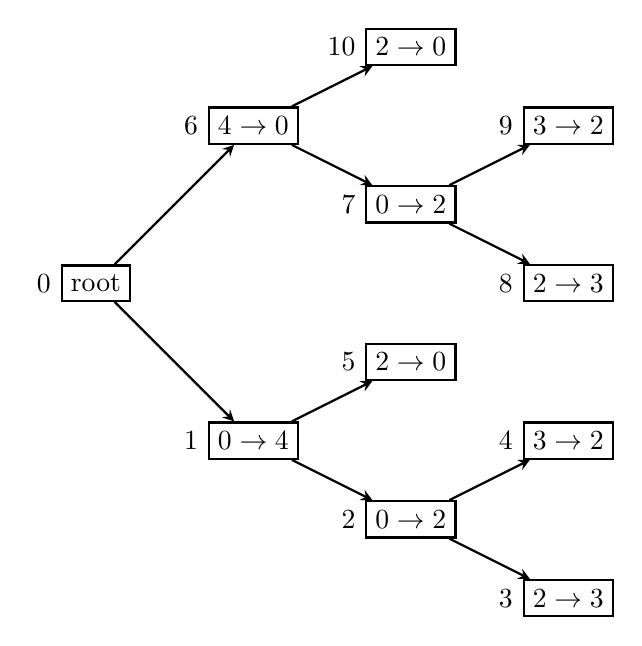
\begin{tikzpicture} [
    edge from parent/.style={draw,-stealth,thick},
    nd/.style={thick, draw=black},
    num/.style={left},
    level distance=2cm,
    level 1/.style={sibling distance=4cm},
    level 2/.style={sibling distance=2cm},
    level 3/.style={sibling distance=2cm}
  ]
  \node[nd] (0) {root} [grow'=right]
  child { node[nd] (6) {\textbf{$4 \rightarrow 0$}}
    child { node[nd] (10) {\textbf{$2 \rightarrow 0$}}
      node[num] at (10.west) {10}
    }
    child { node[nd] (7) {\textbf{$0 \rightarrow 2$}}
      child { node[nd] (9) {\textbf{$3 \rightarrow 2$}}
        node[num] at (9.west) {9}
      }
      child { node[nd] (8) {\textbf{$2 \rightarrow 3$}}
        node[num] at (8.west) {8}
      }
      node[num] at (7.west) {7}
    }
    node[num] at (6.west) {6}
  }
  child { node[nd] (1) {\textbf{$0 \rightarrow 4$}}
    child { node[nd] (5) {\textbf{$2 \rightarrow 0$}}
      node[num] at (5.west) {5}
    }
    child { node[nd] (2) {\textbf{$0 \rightarrow 2$}}
      child { node[nd] (4) {\textbf{$3 \rightarrow 2$}}
        node[num] at (4.west) {4}
      }
      child { node[nd] (3) {\textbf{$2 \rightarrow 3$}}
        node[num] at (3.west) {3}
      }
      node[num] at (2.west) {2}
    }
    node[num] at (1.west) {1}
  };
  \node[num] at (0.west) {0};
\end{tikzpicture}

  }
  \caption{Бинарное дерево обхода частично упорядоченного множества,
  представленного на рис.~\ref{fig:topo-dep}.}
  \label{fig:topo-dep-tree}
\end{figure}

На строках~\ref{alg:line:pright} и~\ref{alg:line:pleft}
алгоритма~\ref{alg:topo-dep} формируются новые частично упорядоченные
множества с дополнительным строгим порядком между зависимыми
операциями: $x <_{p} y$ или $y <_{p} x$. Такой обход удобно
представить в виде бинарного дерева~\cite{binary-tree}, как показано
на рисунке~\ref{fig:topo-dep-tree}. Вершины дерева соответствуют
выбору направления неориентированного ребра, а рядом с каждой
вершиной указан номер шага алгоритма.

\begin{figure}[ht]
  \centerfloat{
    \begin{tikzpicture}[
    node distance=1.5cm and 1cm,
    dag/.style={circle, draw=black, fill=white, inner sep=2pt,
    minimum size=8mm},
    dep/.style={-stealth, thick, dashed},
    order/.style={-stealth, thick},
  ]
  \node[dag] (0) {0};
  \node[dag, right=1.0cm of 0] (1) {1};
  \node[dag, right=1.0cm of 1] (2) {2};

  \draw[order] (0) -- (1);
  \draw[order] (1) -- (2);

  \draw[dep] (2) to[bend right] (0);

\end{tikzpicture}

  }
  \caption{Частично упорядоченное множество на шагах~\textbf{5} и~\textbf{10}.}
  \label{fig:poset-for-node-5-10}
\end{figure}

На рисунке~\ref{fig:topo-dep-tree} представлено дерево, в котором
можно заметить уникальные состояния частично упорядоченного множества
на шагах $5$ и $10$. Во время этих шагов частично упорядоченное
множество выглядит так, как показано на
рисунке~\ref{fig:poset-for-node-5-10}. Этому состоянию соответствует
цикл~\cite{cycle} $0 \rightarrow 1 \rightarrow 2 \rightarrow 0$, что
является некорректным состоянием. Поэтому направление ребра $2
\rightarrow 0$ невозможно, и нет смысла продолжать обход. На данном
примере видно, что направление $2 \rightarrow 0$ заведомо неверное,
так как $0 <_{p} 2$. Таким образом, множество $D$ можно уменьшить,
удалив из него подмножество $D_{order}$ (см.~формулу~\ref{eq:dorder}).

\begin{equation}
  \label{eq:dorder}
  \begin{aligned}
    D_{order} = \{\{x, y\} \in D \mid (x, y) \in E_{order}^{+} \text{ или }
    (y, x) \in E_{order}^{+}\}.
  \end{aligned}
\end{equation}

\begin{figure}[ht]
  \centering
  \centerfloat{
    \begin{tikzpicture}[
    node distance=1.5cm and 1cm,
    stepnode/.style={rectangle, draw=black, dashed, thick, inner sep=5pt, rounded corners=5pt},
    dag/.style={circle, draw=black, fill=white, inner sep=2pt, minimum size=8mm},
    arrow/.style={-stealth, thick},
    dep/.style={thick, dashed, draw=black!50},
    order/.style={-stealth, thick}
]
% Step 1
\node (step1) at (0,7) [stepnode, label={Шаг 2}] {
    \begin{tikzpicture}
      \node[dag] (0) {0};
      \node[dag, below left=1.0 and 0.5cm of 0] (4) {4};
      \node[dag, below right=1.0 and 0.5cm of 0] (1) {1};
      \node[dag, below=1.0cm of 1] (2) {2};
      \node[dag, below=1.0cm of 4] (3) {3};

      \draw[order] (0) -- (1);
      \draw[order] (1) -- (3);
      \draw[order] (1) -- (2);
      \draw[order] (0) -- (4);

      \draw[dep] (0) to[bend right] (2);
      \draw[dep] (2) -- (3);
    \end{tikzpicture}
};

% Step 2
\node (step2) [on grid, stepnode, right=8.0cm of step1, label={Шаг 2.1}] {
    \begin{tikzpicture}[on grid=false]
      \node[dag] (4) {4};
      \node[dag, right=1.0cm of 4] (1) {1};
      \node[dag, below=1.0cm of 1] (2) {2};
      \node[dag, below=1.0cm of 4] (3) {3};

      \draw[order] (1) -- (3);
      \draw[order] (1) -- (2);

      \draw[dep] (2) -- (3);
    \end{tikzpicture}
};

% Step 3
\node (step3) [on grid, stepnode, below=4.0cm of step1, label={Шаг 3}] {
    \begin{tikzpicture}[on grid=false]
      \node[dag] (3) {3};
      \node[dag, right=1.0cm of 3] (2) {2};

      \draw[order] (2) -- (3);
    \end{tikzpicture}
};
% Step 4
\node (step4) [on grid, stepnode, below=2.0cm of step3, label={Шаг 4}] {
    \begin{tikzpicture}[on grid=false]
      \node[dag] (3) {3};
      \node[dag, right=1.0cm of 3] (2) {2};

      \draw[order] (3) -- (2);
    \end{tikzpicture}
};
% Step 2.2
\node (step5) [on grid, stepnode, below=5.0cm of step2, label={Шаг 2.2}] {
    \begin{tikzpicture}[on grid=false]
      \node[dag] (3) {3};
      \node[dag, right=1.0cm of 3] (2) {2};

      \draw[dep] (3) -- (2);
    \end{tikzpicture}
};

% Transitions between steps
\draw[arrow] (step1) -- (step2) node [midway,above,draw=none] {Убираем $min(P)$};
\draw[arrow] (step2) -- (step5) node [midway,right,draw=none] {Убираем $min(P)$};
\draw[arrow] (step5) -- (step3) node [midway,sloped,above,draw=none] {Направляем $2 \rightarrow 3$};
\draw[arrow] (step5) -- (step4) node [midway,sloped,below,draw=none] {Направляем $3 \rightarrow 2$};

\end{tikzpicture}

  }
  \caption{Обзор шага~\textbf{2}.}
  \label{fig:detail-traversal-for-step2}
\end{figure}

Разберём более детально отдельные шаги алгоритма на примере,
представленном на рисунке~\ref{fig:detail-traversal-for-step2}. На
втором шаге мы имеем частично упорядоченное множество, которое
удовлетворяет условию $\forall x \in \min(P), y \in P \mid (x, y)
\not \in D$. Можно удалить минимальное множество $\min(P) = \{0\}$ из
частично упорядоченного множества и перейти к шагу 2.1. Здесь снова
выполняется условие, что никакие элементы минимального подмножества
$\min(P) = \{1, 4\}$ не имеют зависимых операций, поэтому можно
уменьшить частично упорядоченное множество. На шаге 2.2 $\min(P) =
\{2, 3\}$, но $\{2, 3\} \in D$, поэтому вначале необходимо направить
неориентированное ребро. Направляем $2 \rightarrow 3$ и переходим к
шагу 3. Направляем $3 \rightarrow 2$ и переходим к шагу 4.

За один шаг ориентирования рёбер можно обработать сразу несколько
элементов частично упорядоченного множества. При выборе элементов
сохраняется строгий порядок: $0~\rightarrow~1$, $0~\rightarrow~4$, а
любое переупорядочивание элементов без отношения зависимости друг с
другом будет принадлежать одному классу эквивалентности. Поэтому
достаточно рассмотреть только один порядок, например
$0~\rightarrow~1~\rightarrow~4$.

\subsection{Применение к тестовым сценариям TSOTool}

Преимущество обхода частично упорядоченного множества с учётом
зависимостей (алгоритм~\ref{alg:topo-dep}) наглядно проявляется на
тестовых сценариях инструмента TSOTool (см. раздел~\ref{sec:manovit}).

Частично упорядоченное множество определяется моделью памяти. Если
результат операции $b$ не может наблюдаться до выполнения операции
$a$, то $a < b$. Пара ``адрес/значение'' задаёт отношение зависимости
между операциями. Условие уникальности пар ``адрес/значение'' при
верификации с использованием алгоритма~\ref{alg:topo-dep} однозначно
определяет порядок между операциями в момент выбора направления (либо
$P^{\rightarrow}$, либо $P^{\leftarrow}$).

\begin{figure}[ht]
  \centering
  \centerfloat{
    % This file was created with tikzplotlib v0.10.1.post13.
\begin{tikzpicture}

  \definecolor{darkgrey176}{RGB}{176,176,176}
  \definecolor{lightgrey204}{RGB}{204,204,204}

  \begin{axis}[
      height=0.4\textheight,
      legend cell align=right,
      legend pos=north west,
      legend style={  at={(1,1.03)},  anchor=south east},
      tick align=outside,
      tick pos=left,
      width=0.95\textwidth,
      x grid style={darkgrey176},
      xlabel={\(\displaystyle |P|, шт\)},
      xmin=6800, xmax=33200,
      xtick style={color=black},
      y grid style={darkgrey176},
      ylabel style={text width=10cm, align=center},
      ylabel={Время, мс},
      ymin=-275.5095, ymax=5785.6995,
      ytick style={color=black}
    ]
    \path [draw=black, semithick]
    (axis cs:8000,0)
    --(axis cs:8000,261.365);

    \addplot [semithick, black, mark=*, mark size=3, mark
    options={solid}, only marks]
    table {%
      8000 261.365
    };
    \addplot [semithick, red]
    table {%
      8000 0
      8000 0
    };
    \path [draw=black, semithick]
    (axis cs:12000,0)
    --(axis cs:12000,638.937);

    \addplot [semithick, black, mark=*, mark size=3, mark
    options={solid}, only marks]
    table {%
      12000 638.937
    };
    \addplot [semithick, red]
    table {%
      12000 0
      12000 0
    };
    \path [draw=black, semithick]
    (axis cs:16000,0)
    --(axis cs:16000,1137.16);

    \addplot [semithick, black, mark=*, mark size=3, mark
    options={solid}, only marks]
    table {%
      16000 1137.16
    };
    \addplot [semithick, red]
    table {%
      16000 0
      16000 0
    };
    \path [draw=black, semithick]
    (axis cs:20000,0)
    --(axis cs:20000,1866.19);

    \addplot [semithick, black, mark=*, mark size=3, mark
    options={solid}, only marks]
    table {%
      20000 1866.19
    };
    \addplot [semithick, red]
    table {%
      20000 0
      20000 0
    };
    \path [draw=black, semithick]
    (axis cs:24000,0)
    --(axis cs:24000,2700.01);

    \addplot [semithick, black, mark=*, mark size=3, mark
    options={solid}, only marks]
    table {%
      24000 2700.01
    };
    \addplot [semithick, red]
    table {%
      24000 0
      24000 0
    };
    \path [draw=black, semithick]
    (axis cs:28000,0)
    --(axis cs:28000,4113.57);

    \addplot [semithick, black, mark=*, mark size=3, mark
    options={solid}, only marks]
    table {%
      28000 4113.57
    };
    \addplot [semithick, red]
    table {%
      28000 0
      28000 0
    };
    \path [draw=black, semithick]
    (axis cs:32000,0)
    --(axis cs:32000,5510.19);

    \addplot [semithick, black, mark=*, mark size=3, mark
    options={solid}, only marks]
    table {%
      32000 5510.19
    };
    \addplot [semithick, red]
    table {%
      32000 0
      32000 0
    };
  \end{axis}

\end{tikzpicture}

  }
  \caption{График времени построения одного линейного порядка в
  зависимости от количества элементов множества. $p_{P} = 0.001$.}
  \label{fig:manovit-exp}
  % ./build/examples/example --algorithm dep --nodes 28000
  % --poset-edge-prob 0.001 --dependency-edge-prob 0.3 --seed 0
  % --predefined 3 --linexts-act print-one
  % ./scripts/manovit-exp.py --nds 8000 12000 16000 20000 24000 28000
  % 32000 --pepr 0.001 --experiments 1 --only-max --not-continue
\end{figure}

Промоделируем эксперимент с графом, получаемым инструментом TSOTool.
Предположим, что половина всех операций с памятью — это операции
чтения, а другая половина — операции записи. Во время верификации
цикл между операциями $M[x] == v$ и $M[x] := v$ возможен только в
случае некорректного поведения тестируемой системы.
Алгоритм~\ref{alg:topo-dep} допускает циклы, если возможны другие
порядки чтения/записи, однако в контексте построения псевдослучайного
теста такие порядки невозможны. Для моделирования отсутствия циклов
используем сильно разреженное частично упорядоченное множество с
параметром $p_{P} = 0.001$. Уникальность пар ``адрес/значение''
моделируется наличием только одного ребра между операцией чтения и
операцией записи.

На графике~\ref{fig:manovit-exp} представлены результаты построения
одного порядка в зависимости от количества элементов множества. Как
видно, обход с учётом зависимостей может применяться для проверки
нескольких тысяч операций с памятью.

\subsection{Асимптотика алгоритма построения всех линейных порядков
топологической сортировкой с учётом зависимости}
\label{sec:ch2/dep-comp}

Так как порядок определяется путём выбора направления
неориентированного ребра из $E_{dep}$, то количество направлений
равно $2^{|D|}$, асимптотическая сложность алгоритма задаётся
соотношением~\ref{eq:ass}, где $D$ — множество зависимых элементов,
$n$ — количество элементов частично упорядоченного множества.

\begin{equation}
  O(2^{|D|}n^2),
  \label{eq:ass}
\end{equation}

\fixme{move verbose/detailed??}
\fixme{не переносить формулы}

Возможны случаи, когда $\exists \{x, y\} \in D \mid x <_{p} y$.
То есть зависимые элементы обладают отношением порядка.
В этом случае нет смысла строить $P^{\leftarrow} = P \cup (y <_{p}
x)$, так как оно заведомо будет обладать циклом.
Множество $D$ можно минимизировать из условия $D_{min} = \{\{x, y\}
\in D \mid x \not <_{p} y \land y \not <_{p} x \}$.
Общее количество перестановок не изменится, так как цикл обработается
на строке 3 листинга~\ref{alg:topo-dep}, однако уменьшение множества
$D$ уменьшает показатель степени в формуле~\ref{eq:ass}.

\section{Сравнение алгоритмов построения линейных
порядков}\label{sec:ch2/indep-dep}

Все представленные алгоритмы
обхода~\ref{alg:topo},~\ref{alg:topo-indep},~\ref{alg:topo-indep-lookup},~\ref{alg:topo-dep}
имеют одинаковую асимптотическую сложность в общем случае.
Но
алгоритмы~\ref{alg:topo-indep},~\ref{alg:topo-indep-lookup},~\ref{alg:topo-dep},
учитывающие классы эквивалентности, существенно уменьшают количество
линейных порядков, необходимых для анализа.
Сравнение количества линейных порядков случайных частично
упорядоченных множеств с учётом эквивалентности и без неё
представлено в таблице~\ref{tb:table}.
Общее количество линейных порядков было рассчитано с помощью
алгоритма, описанного в работе~\cite{poset}.
Количество линейных порядков с учётом эквивалентности рассчитано
алгоритмом~\ref{alg:topo-indep}.

\begin{table}[ht]
  \captionsetup{justification=raggedright,singlelinecheck=false}
  \caption{Сравнение количества линейных порядков.}
  \centering
  \begin{tabular}{|c|c|c|}
    \hline
    \textbf{Размер множества} & \textbf{
      \begin{tabular}[c]{@{}c@{}}Общее количество \\ линейных порядков
    \end{tabular}} & \textbf{
      \begin{tabular}[c]{@{}c@{}}Количество линейных порядков с
        \\ учётом эквивалентности
    \end{tabular}} \\ \hline
    4                        & 12                                 & 3
    \\ \hline
    9                        & 105                                &
    20
    \\ \hline
    16                       & 2041200                            &
    196
    \\ \hline
    20                       & 1036062752256                      &
    38433
    \\ \hline
    28                       & 6587142659584819200                &
    61881
    \\ \hline
  \end{tabular}\label{tb:table}
\end{table}

При построении таблицы~\ref{tb:table} были выбраны такие множества, в
которых количество рёбер эквивалентности близко к количеству
элементов в частично упорядоченном множестве: $|B^|| \sim |P|$.

Некоторые дальнейшие результаты не будут включать алгоритм обхода
топологической сортировкой~\ref{alg:topo}, так как полный обход всех
линейных порядков не может быть произведён за разумное время.
Без эвристики эквивалентности количество линейных порядков в худшем
случае может достигать $n!$.
Преимуществом алгоритмов, учитывающих эквивалентность, является то,
что в некоторых пределах асимптотическая сложность данных алгоритмов
может приближаться к $O(n^2)$
(см.~\ref{eq:topo-indep-comp-lims},~\ref{eq:ass}).

Обозначим $p_{D}$ -- вероятность зависимости между элементами множества $P$.
\begin{equation}
  p_{D} = p_{D}(x, y) = \mathbb{P}[ \{x, y\} \in D ],\ \forall x, y \in P
  \label{eq:prob_dep}
\end{equation}

И $p_{P}$ -- вероятность отношения порядка между элементами множества $P$.
\begin{equation}
  p_{P} = p_{P}(x, y) = \mathbb{P}[x <_{p} y],\ \forall x, y \in P
  \label{eq:prob_pos}
\end{equation}

\begin{figure}[ht]
  \centering
  \centerfloat{
    % This file was created with tikzplotlib v0.10.1.post13.
\begin{tikzpicture}

\definecolor{darkgrey176}{RGB}{176,176,176}
\definecolor{green}{RGB}{0,128,0}
\definecolor{lightgrey}{RGB}{211,211,211}
\definecolor{lightgrey204}{RGB}{204,204,204}
\definecolor{orange}{RGB}{255,165,0}

\begin{axis}[
height=0.4\textheight,
legend cell align=right,
legend pos=north west,
legend style={  at={(1,1.03)},  anchor=south east},
tick align=outside,
tick pos=left,
width=0.95\textwidth,
x grid style={darkgrey176},
xlabel={Вероятность зависимости между элементами, \(\displaystyle p_{D}\)},
xmin=-0.0665, xmax=1.0665,
xtick style={color=black},
y grid style={darkgrey176},
ylabel style={text width=10cm, align=center},
ylabel={Количество линейных перестановок
в логарифмическом масштабе, \(\displaystyle log_{10}(\text{шт})\)},
ymin=0, ymax=7.01323097713965,
ytick style={color=black}
]
\draw[draw=black,fill=orange] (axis cs:0.005,0) rectangle (axis cs:0.015,0);
\addlegendimage{ybar,ybar legend,draw=black,fill=orange}
\addlegendentry{Обход с учётом зависимости, Алгоритм~\ref{alg:topo-dep}}

\draw[draw=black,fill=orange] (axis cs:0.105,0) rectangle (axis cs:0.115,2.15836249209525);
\draw[draw=black,fill=orange] (axis cs:0.205,0) rectangle (axis cs:0.215,3.2895889525426);
\draw[draw=black,fill=orange] (axis cs:0.305,0) rectangle (axis cs:0.315,3.74083620705731);
\draw[draw=black,fill=orange] (axis cs:0.405,0) rectangle (axis cs:0.415,4.57801998503221);
\draw[draw=black,fill=orange] (axis cs:0.505,0) rectangle (axis cs:0.515,4.88829746216554);
\draw[draw=black,fill=orange] (axis cs:0.605,0) rectangle (axis cs:0.615,5.21851712477091);
\draw[draw=black,fill=orange] (axis cs:0.705,0) rectangle (axis cs:0.715,5.58294243056767);
\draw[draw=black,fill=orange] (axis cs:0.805,0) rectangle (axis cs:0.815,5.9647525881337);
\draw[draw=black,fill=orange] (axis cs:0.905,0) rectangle (axis cs:0.915,6.28133522204542);
\draw[draw=black,fill=orange] (axis cs:1.005,0) rectangle (axis cs:1.015,6.60437381770785);
\draw[draw=black,fill=white] (axis cs:-0.015,0) rectangle (axis cs:-0.005,4.63578523553365);
\addlegendimage{ybar,ybar legend,draw=black,fill=white}
\addlegendentry{Обход с учётом независимости, Алгоритм~\ref{alg:topo-indep}}

\draw[draw=black,fill=white] (axis cs:0.085,0) rectangle (axis cs:0.095,4.78859255592036);
\draw[draw=black,fill=white] (axis cs:0.185,0) rectangle (axis cs:0.195,4.91948080530445);
\draw[draw=black,fill=white] (axis cs:0.285,0) rectangle (axis cs:0.295,5.118215108501);
\draw[draw=black,fill=white] (axis cs:0.385,0) rectangle (axis cs:0.395,5.44137145388074);
\draw[draw=black,fill=white] (axis cs:0.485,0) rectangle (axis cs:0.495,5.56050560995127);
\draw[draw=black,fill=white] (axis cs:0.585,0) rectangle (axis cs:0.595,5.71155501203113);
\draw[draw=black,fill=white] (axis cs:0.685,0) rectangle (axis cs:0.695,5.88895076288752);
\draw[draw=black,fill=white] (axis cs:0.785,0) rectangle (axis cs:0.795,6.13416817925776);
\draw[draw=black,fill=white] (axis cs:0.885,0) rectangle (axis cs:0.895,6.3165498571675);
\draw[draw=black,fill=white] (axis cs:0.985,0) rectangle (axis cs:0.995,6.60437381770785);
\draw[draw=black,fill=green] (axis cs:-0.005,0) rectangle (axis cs:0.005,0);
\addlegendimage{ybar,ybar legend,draw=black,fill=green}
\addlegendentry{Обход с учётом независимости, Алгоритм~\ref{alg:topo-indep-lookup}}

\draw[draw=black,fill=green] (axis cs:0.095,0) rectangle (axis cs:0.105,2.15836249209525);
\draw[draw=black,fill=green] (axis cs:0.195,0) rectangle (axis cs:0.205,3.2895889525426);
\draw[draw=black,fill=green] (axis cs:0.295,0) rectangle (axis cs:0.305,3.74083620705731);
\draw[draw=black,fill=green] (axis cs:0.395,0) rectangle (axis cs:0.405,4.57801998503221);
\draw[draw=black,fill=green] (axis cs:0.495,0) rectangle (axis cs:0.505,4.88829746216554);
\draw[draw=black,fill=green] (axis cs:0.595,0) rectangle (axis cs:0.605,5.21851712477091);
\draw[draw=black,fill=green] (axis cs:0.695,0) rectangle (axis cs:0.705,5.58294243056767);
\draw[draw=black,fill=green] (axis cs:0.795,0) rectangle (axis cs:0.805,5.9647525881337);
\draw[draw=black,fill=green] (axis cs:0.895,0) rectangle (axis cs:0.905,6.28133522204542);
\draw[draw=black,fill=green] (axis cs:0.995,0) rectangle (axis cs:1.005,6.60437381770785);
\addplot [semithick, red, dash pattern=on 1pt off 3pt on 3pt off 3pt]
table {%
-0.0665 6.60437381770785
1.0665 6.60437381770785
};
\addlegendentry{Обход топологической сортировкой, Алгоритм~\ref{alg:topo}}
\addplot [semithick, lightgrey]
table {%
0 0.17129391428814
0.1 1.90632082152951
0.2 3.14208626146731
0.3 3.98780434183084
0.4 4.5526891703494
0.5 4.94595485475229
0.6 5.26496572446256
0.7 5.55968699567826
0.8 5.86823410629118
0.9 6.22872249419311
1 6.67926759727586
};
\end{axis}

\end{tikzpicture}

  }
  % ./scripts/launch_experiments.py --nds 13 --y-axis=linext
  % --only-max --not-continue --in-log --to-tex
  \caption{График зависимости количества линейных порядков в
    логарифмическом масштабе от вероятности зависимости элементов для
  обходов с учётом зависимости и независимости. $|P| = 13$, $p_{P} = 0.3$.}
  \label{fig:nds-13-linext}
\end{figure}

Из формулы~\ref{eq:supset} следует, что количество линейных порядков
при обходе с учётом $B$ всегда меньше либо равно количеству линейных
порядков при обходе с учётом $B^|$.
Кроме того, по построению, количество линейных порядков всегда равно
количеству классов эквивалентности, что означает минимальное
возможное количество для данного частично упорядоченного множества.
На графике~\ref{fig:nds-13-linext} показано, что количество линейных
порядков для одной и той же конфигурации частично упорядоченного
множества меньше при обходе с учётом зависимостей, по сравнению с
обходом с учётом независимостей.
Красной линией обозначено максимально возможное количество линейных
порядков для данной конфигурации частично упорядоченного множества.

\begin{figure}[ht]
  \centering
  \centerfloat{
    % This file was created with tikzplotlib v0.10.1.post13.
\begin{tikzpicture}

  \definecolor{darkgrey176}{RGB}{176,176,176}
  \definecolor{green}{RGB}{0,128,0}
  \definecolor{lightgrey}{RGB}{211,211,211}
  \definecolor{lightgrey204}{RGB}{204,204,204}
  \definecolor{orange}{RGB}{255,165,0}

  \begin{axis}[
      height=0.4\textheight,
      legend cell align=right,
      legend pos=north west,
      legend style={  at={(1,1.03)},  anchor=south east},
      tick align=outside,
      tick pos=left,
      width=0.95\textwidth,
      x grid style={darkgrey176},
      xlabel={Вероятность зависимости между элементами,
      \(\displaystyle p_{D}\)},
      xmin=-0.0665, xmax=1.0665,
      xtick style={color=black},
      y grid style={darkgrey176},
      ylabel style={text width=10cm, align=center},
      ylabel={Время
      в логарифмическом масштабе, \(\displaystyle log_{10}(\text{мс} * 100)\)},
      ymin=0, ymax=6.45493824874219,
      ytick style={color=black}
    ]
    \draw[draw=black,fill=orange] (axis cs:0.005,0) rectangle (axis
    cs:0.015,0.672698063024046);
    \addlegendimage{ybar,ybar legend,draw=black,fill=orange}
    \addlegendentry{Обход с учётом зависимости, Алгоритм~\ref{alg:topo-dep}}

    \draw[draw=black,fill=orange] (axis cs:0.105,0) rectangle (axis
    cs:0.115,2.200896988085);
    \draw[draw=black,fill=orange] (axis cs:0.205,0) rectangle (axis
    cs:0.215,3.10438808634469);
    \draw[draw=black,fill=orange] (axis cs:0.305,0) rectangle (axis
    cs:0.315,3.30237422607558);
    \draw[draw=black,fill=orange] (axis cs:0.405,0) rectangle (axis
    cs:0.415,4.16833245562574);
    \draw[draw=black,fill=orange] (axis cs:0.505,0) rectangle (axis
    cs:0.515,4.46480837004647);
    \draw[draw=black,fill=orange] (axis cs:0.605,0) rectangle (axis
    cs:0.615,4.75409670845534);
    \draw[draw=black,fill=orange] (axis cs:0.705,0) rectangle (axis
    cs:0.715,5.12614440017105);
    \draw[draw=black,fill=orange] (axis cs:0.805,0) rectangle (axis
    cs:0.815,5.48329053467323);
    \draw[draw=black,fill=orange] (axis cs:0.905,0) rectangle (axis
    cs:0.915,5.80480570279117);
    \draw[draw=black,fill=orange] (axis cs:1.005,0) rectangle (axis
    cs:1.015,6.07932598675282);
    \draw[draw=black,fill=white] (axis cs:-0.015,0) rectangle (axis
    cs:-0.005,3.91260621327443);
    \addlegendimage{ybar,ybar legend,draw=black,fill=white}
    \addlegendentry{Обход с учётом независимости, Алгоритм~\ref{alg:topo-indep}}

    \draw[draw=black,fill=white] (axis cs:0.085,0) rectangle (axis
    cs:0.095,4.03298119309737);
    \draw[draw=black,fill=white] (axis cs:0.185,0) rectangle (axis
    cs:0.195,4.13142296322114);
    \draw[draw=black,fill=white] (axis cs:0.285,0) rectangle (axis
    cs:0.295,4.27295494484817);
    \draw[draw=black,fill=white] (axis cs:0.385,0) rectangle (axis
    cs:0.395,4.47818686310984);
    \draw[draw=black,fill=white] (axis cs:0.485,0) rectangle (axis
    cs:0.495,4.60648992516164);
    \draw[draw=black,fill=white] (axis cs:0.585,0) rectangle (axis
    cs:0.595,4.72960453322533);
    \draw[draw=black,fill=white] (axis cs:0.685,0) rectangle (axis
    cs:0.695,4.87760686083614);
    \draw[draw=black,fill=white] (axis cs:0.785,0) rectangle (axis
    cs:0.795,5.09484132652886);
    \draw[draw=black,fill=white] (axis cs:0.885,0) rectangle (axis
    cs:0.895,5.32629693656581);
    \draw[draw=black,fill=white] (axis cs:0.985,0) rectangle (axis
    cs:0.995,5.52179034348834);
    \draw[draw=black,fill=green] (axis cs:-0.005,0) rectangle (axis
    cs:0.005,2.60540848858583);
    \addlegendimage{ybar,ybar legend,draw=black,fill=green}
    \addlegendentry{Обход с учётом независимости,
    Алгоритм~\ref{alg:topo-indep-lookup}}

    \draw[draw=black,fill=green] (axis cs:0.095,0) rectangle (axis
    cs:0.105,3.17469347914945);
    \draw[draw=black,fill=green] (axis cs:0.195,0) rectangle (axis
    cs:0.205,3.39158253515756);
    \draw[draw=black,fill=green] (axis cs:0.295,0) rectangle (axis
    cs:0.305,3.88808902988961);
    \draw[draw=black,fill=green] (axis cs:0.395,0) rectangle (axis
    cs:0.405,4.20617259446969);
    \draw[draw=black,fill=green] (axis cs:0.495,0) rectangle (axis
    cs:0.505,4.40737900582878);
    \draw[draw=black,fill=green] (axis cs:0.595,0) rectangle (axis
    cs:0.605,4.64942054065054);
    \draw[draw=black,fill=green] (axis cs:0.695,0) rectangle (axis
    cs:0.705,4.89481322245816);
    \draw[draw=black,fill=green] (axis cs:0.795,0) rectangle (axis
    cs:0.805,5.13628288216488);
    \draw[draw=black,fill=green] (axis cs:0.895,0) rectangle (axis
    cs:0.905,5.3313847760984);
    \draw[draw=black,fill=green] (axis cs:0.995,0) rectangle (axis
    cs:1.005,5.4919762757976);
    \addplot [semithick, lightgrey]
    table {%
      0 0.813095484880913
      0.1 2.01027690596296
      0.2 2.91956692726929
      0.3 3.59800273858807
      0.4 4.10262152970745
      0.5 4.49046049041558
      0.6 4.8143432165528
      0.7 5.11023892816826
      0.8 5.40990325136328
      0.9 5.74509181223919
      1 6.14756023689733
    };
  \end{axis}

\end{tikzpicture}

  }
  % ./scripts/launch_experiments.py --nds 13 --y-axis=time --only-max
  % --not-continue --in-log --to-tex
  \caption{График зависимости времени построения линейных порядков в
    логарифмическом масштабе от вероятности зависимости элементов для
  обходов с учётом зависимости и независимости. $|P| = 13$, $p_{P} = 0.3$.}
  \label{fig:nds-13-time}
\end{figure}

\section{Выводы по главе~\ref{sec:ch3}}

В главе для снижения вычислительной сложности предложено использовать
свойство независимости операций с памятью. Две операции названы
независимыми, если любой порядок их исполнения приводит систему в
одно и то же состояние. На основе этого свойства введены классы
эквивалентных перестановок и построено разбиение $B^∣$.

Разработан алгоритм топологической сортировки с учётом независимости
(алгоритм~\ref{alg:topo-indep}), который исключает из обхода
эквивалентные перестановки соседних независимых элементов. Доказана
лемма о возможности перестановки элемента с подпорядком независимых
элементов любой длины (лемма~\ref{lm:n-reorder}). На её основе
предложен модифицированный алгоритм
(алгоритм~\ref{alg:topo-indep-lookup}), обеспечивающий полный учёт
эквивалентных перестановок.

Получена асимптотическая оценка сложности алгоритма с учётом
независимости. Показано, что при высокой вероятности независимости
элементов ($p_i \approx 1$) сложность алгоритма снижается до $O(n^2)$,
что существенно лучше общего случая. Таким образом, предложенный
подход позволяет значительно сократить количество анализируемых
линейных порядков в программах с большим числом независимых операций.
В дополнения к анализу независимых операций, было введено понятие
зависимых операций (определение~\ref{def:dep}) и предложен алгоритм
построения линейных порядков
с учётом зависимости (алгоритм~\ref{alg:topo-dep}).
Асимптотическая сложность данного подхода равна $O(2^{|D|}n^2)$, где
$D$ -- множество независимых операций.
Таким образом, малое количество зависимых операций уменьшает
показатель степени в
асимптотической оценке.

Экспериментально подтверждена применимость алгоритма с учётом
зависимости для проверки нескольких тысяч операций с памятью в
сценариях, моделирующих работу инструмента TSOTool.

Проведено сравнение разработанных алгоритмов. Показано, что
алгоритмы, учитывающие классы эквивалентности (независимость и
зависимость), существенно сокращают количество линейных порядков,
необходимых для анализа, по сравнению с полным обходом. При этом
они обеспечивают минимальное возможное
количество линейных порядков для данного частично упорядоченного
множества, что подтверждается как теоретическими оценками, так и
экспериментальными данными (таблица~\ref{tb:table},
рисунки~\ref{fig:nds-13-linext}~и~\ref{fig:nds-13-time}).

Таким образом, предложенные в главе подходы позволяют эффективно
решать задачу построения линейных порядков для частично упорядоченных
множеств операций с памятью, используя свойства многопоточных программ.
Полученные результаты являются основой для разработки методов
верификации подсистемы памяти, учитывающих как модель памяти, так и
зависимости между операциями.
Вместе с тем, экспоненциальный рост числа состояний и сложности их
верификации обосновывает необходимость разработки специализированной
структуры данных для компактного хранения результатов обхода, что
будет представлено в следующей главе.

\clearpage
